\documentclass[10pt,french]{book}
\input preambule_2013

\newcounter{exoc}
\newenvironment{exoc}[1]{%
  \refstepcounter{exoc}\textbf{Exercice \theexoc} :\hfill {\textbf{(#1)}}\par
  \medskip}%
{\medskip}

\pagestyle{empty}

\newcommand\Kdo[1][1em]{$
\includegraphics[width=10pt]{kdo.eps}\hspace{#1}$}
\newcommand\Red[1][1em]{$\includegraphics[width=10pt]{bc-crayon}\hspace{#1}$}

\begin{document}

\begin{center}
\begin{tabularx}{\textwidth}{|>\centering m{2.5cm}|>\centering X|>{\centering\arraybackslash} m{2.5cm}|}
	\hline
		\seconde 7 &  Mardi 28 janvier \np{2014} & \textbf{Statistiques discrètes} \\
	\hline
		\multicolumn{3}{|c|}{\bsc{Contrôle de mathématiques}} \\
	\hline
        \multicolumn{1}{|r}{\bsc{Nom}:} & \multicolumn{2}{l|}{} \\
		\multicolumn{1}{|r}{Prénom:} & \multicolumn{2}{l|}{} \\
	\hline
        \multicolumn{3}{|l|}{\bfseries Note et observations :} \\[1cm]
    \hline
\end{tabularx}\medskip

{\itshape
\small
Le barème est indicatif. Répondre aux questions \textbf{par des phrases}.\par
{\bfseries Les questions \Red[0pt] demandent une rédaction plus précise et plus appliquée.}\par
Les questions \Kdo[0pt] doivent absolument être réussie.
}
\end{center}



\begin{exoc}{8,5 points}
    On a étudié la répartition du nombre de frères et s{\oe}urs des élèves d'une classe puis on a établi le tableau suivant :
    \begin{center}
        \renewcommand\arraystretch{2}
        \begin{tabularx}{0.75\linewidth}{|>{\centering\bfseries} m{2.5cm}|*{6}{>{\centering\arraybackslash}X|}}
            \hline
                Nombre de frères et s{oeu}rs & $0$ & $1$ & $2$ & $3$ & $4$ & $5$ \\
            \hline
                Effectif & $5$ &$7$ & $10$ & $5$ & $4$ & $3$ \\
            \hline
                Effectif Cumulé Croissant & & & & & & \\
            \hline
        \end{tabularx}
    \end{center}
    
    \begin{enumerate}
        \item \Kdo Combien y a t'il d'élèves dans la classe ? \hfill \textbf{/0,5}
        \item Compléter la dernière ligne du tableau. \hfill \textbf{/0,5}
        \item Quel est le pourcentage d'enfants uniques dans la classe ? \hfill \textbf{/1}
        \item \Kdo Calculer l'étendue de cette série statistique. \hfill \textbf{/0,5}
        \item Calculer le nombre moyen de frères et s{\oe}urs par élève dans cette classe. \hfill \textbf{/1}
        \item \Red Déterminer une médiane de cette série statistique. Interpréter le résultat. \hfill \textbf{/1,5}
        \item \Red Déterminer le premier et le troisième quartile de cette série statistique. Interpréter les résultats. \hfill \textbf{/3}
        \item Représenter ci-dessous le diagramme en bâton de la série statistique. \hfill \textbf{/0,5}
    \end{enumerate}
    
    \begin{center}
        
\begin{tikzpicture}[scale=0.75]
            \draw[help lines] (-0.5,-0.5) grid (13.5,10.5);
            \draw[<->] (0,11)--(0,0)--(14,0);
        \end{tikzpicture}
    \end{center}
\end{exoc}\clearpage

\begin{exoc}{6,5 points}
    On considère les deux séries statistiques ci-dessous représentant les adolescents d'un club de sport en fonction de leur âge.\par
    La série de gauche représente la répartition des garçons et la série de droite celle des filles.\medskip

    \begin{center}
        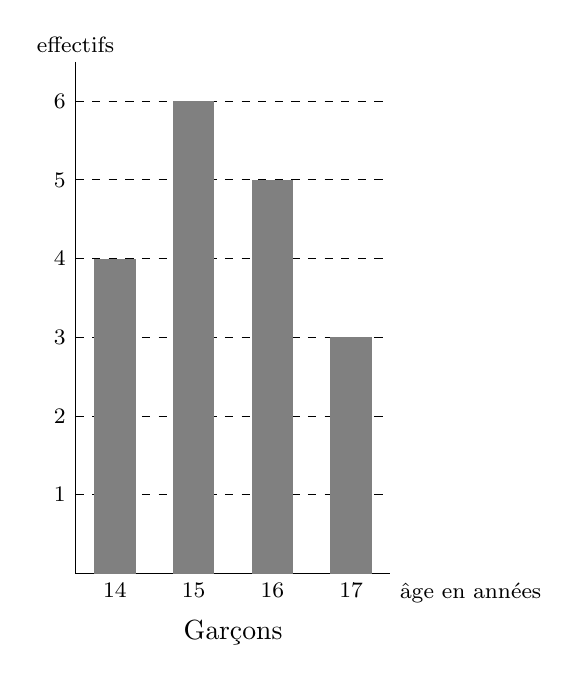
\begin{tikzpicture}
            \foreach \x in {1,2,3,4,5,6} \draw[dashed] (0,\x) -- (4,\x);
            \foreach \x in {1,2,3,4,5,6} \draw (0,\x) node[left] {\footnotesize $\x$};
            \draw[line width = 0.2pt] (0,6.5) node[above] {\footnotesize effectifs} -- (0,0) -- (4,0) node[below right] {\footnotesize âge en années};
            \draw[line width = 15pt,color=gray] (0.5,0) -- (0.5,4);
            \draw[line width = 15pt,color=gray] (1.5,0) -- (1.5,6);
            \draw[line width = 15pt,color=gray] (2.5,0) -- (2.5,5);
            \draw[line width = 15pt,color=gray] (3.5,0) -- (3.5,3);
            \foreach \x in {14,15,16,17} \draw (\x-13.5,0) node[below] {\footnotesize $\x$};
            \draw (2,-0.75) node {\bsc{Garçons}};
        \end{tikzpicture}
        \hspace*{2cm}
        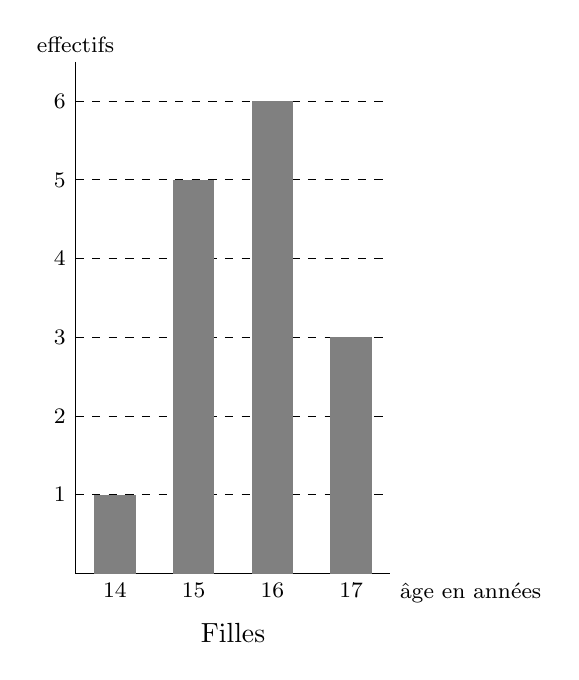
\begin{tikzpicture}
            \foreach \x in {1,2,3,4,5,6} \draw[dashed] (0,\x) -- (4,\x);
            \foreach \x in {1,2,3,4,5,6} \draw (0,\x) node[left] {\footnotesize $\x$};
            \draw[line width = 0.2pt] (0,6.5) node[above] {\footnotesize effectifs} -- (0,0) -- (4,0) node[below right] {\footnotesize âge en années};
            \draw[line width = 15pt,color=gray] (0.5,0) -- (0.5,1);
            \draw[line width = 15pt,color=gray] (1.5,0) -- (1.5,5);
            \draw[line width = 15pt,color=gray] (2.5,0) -- (2.5,6);
            \draw[line width = 15pt,color=gray] (3.5,0) -- (3.5,3);
            \foreach \x in {14,15,16,17} \draw (\x-13.5,0) node[below] {\footnotesize $\x$};
            \draw (2,-0.75) node {\bsc{Filles}};
        \end{tikzpicture}
    \end{center}

    \begin{enumerate}
        \item \Kdo Combien y a t-il de garçons dans le club ? Justifier en écrivant le calcul effectué. \hfill \textbf{/0,5}
        \item \Red Déterminer une médiane de la série statistiques des garçons et interpréter le résultat. \hfill \textbf{/1,5}
        \item \Kdo Combien y a t-il de filles dans le club ? Justifier en écrivant le calcul effectué. \hfill \textbf{/0,5}
        \item \Red Déterminer une médiane de la série statistiques des filles et interpréter le résultat. \hfill \textbf{/1,5}
        \item En détaillant précisément le calcul, calculer l'âge moyen d'un adolescent pour l'ensemble du club. \hfill \textbf{/1}
        \item \Red En détaillant précisément les étapes, déterminer l'âge médian de l'ensemble des adolescents du club de sport. Interpréter le résultat. \hfill \textbf{/1,5}
    \end{enumerate}
\end{exoc}
\[*\]

\begin{exoc}{DNB juin 2013 - France métropolitaine - 5 points}

Les informations suivantes concernent les salaires des hommes et des femmes d'une même entreprise :
\medskip

\begin{tabularx}{\linewidth}{|>{\centering \arraybackslash}X|}\hline
\textbf{Salaires des femmes :}\\
\np{1200}~\euro{} ; \np{1230}~\euro{} ; \np{1250}~\euro{} ; \np{1310}~\euro{} ; \np{1376}~\euro{} ; \np{1400}~\euro{} ; \np{1440}~\euro{} ; \np{1500}~\euro{} ; \np{1700}~\euro{} ; \np{2100}~\euro{}\\ \hline
\end{tabularx}

\medskip

\begin{tabularx}{\linewidth}{|>{\centering \arraybackslash}X|}\hline
\textbf{Salaires des hommes :} \\
Effectif total : 20\\
Moyenne : \np{1769}~\euro\\
Étendue: \np{2400}~\euro \\
Médiane: \np{2000}~\euro\\
Les salaires des hommes sont tous différents.\\ \hline
\end{tabularx}

\medskip

\begin{enumerate}
\item Comparer le salaire moyen des hommes et celui des femmes. \hfill \textbf{/1}
\item \Red Le plus bas salaire de l'entreprise est de \np{1000}~\euro. Quel salaire est le plus élevé ? Justifier la réponse. \hfill \textbf{/2}
\item \Red Dans cette entreprise combien de personnes gagnent plus de \EUR{$\np{2000}$} ? Justifier la réponse. \hfill \textbf{/2}
\end{enumerate}
\end{exoc}

\end{document} 